%% AUTO-GENERATED by family_report/generate_latex.py — do not edit.
\begin{figure}[t]\centering
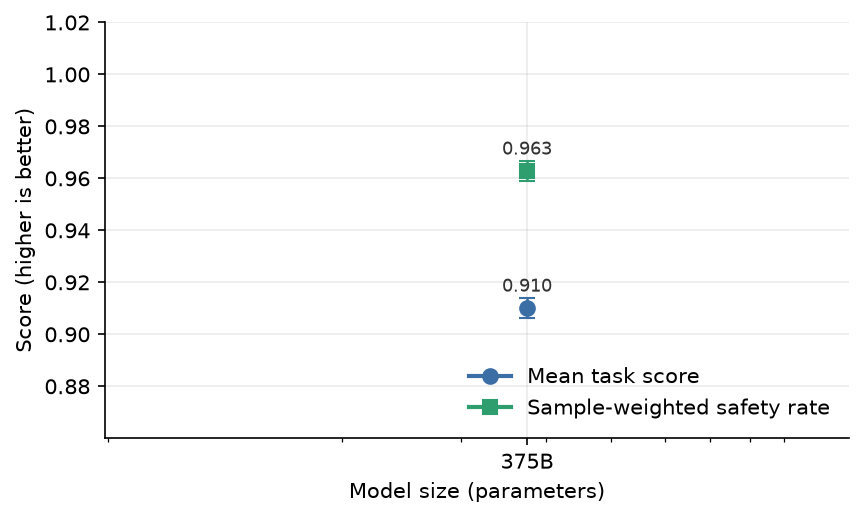
\includegraphics[width=\linewidth]{figures/fam_scaling_overall.png}
\caption{Overall safety vs.\ model size: main-suite mean score and sample-weighted safety rate.}
\label{fig:fam-scaling}
\end{figure}

\begin{figure}[t]\centering
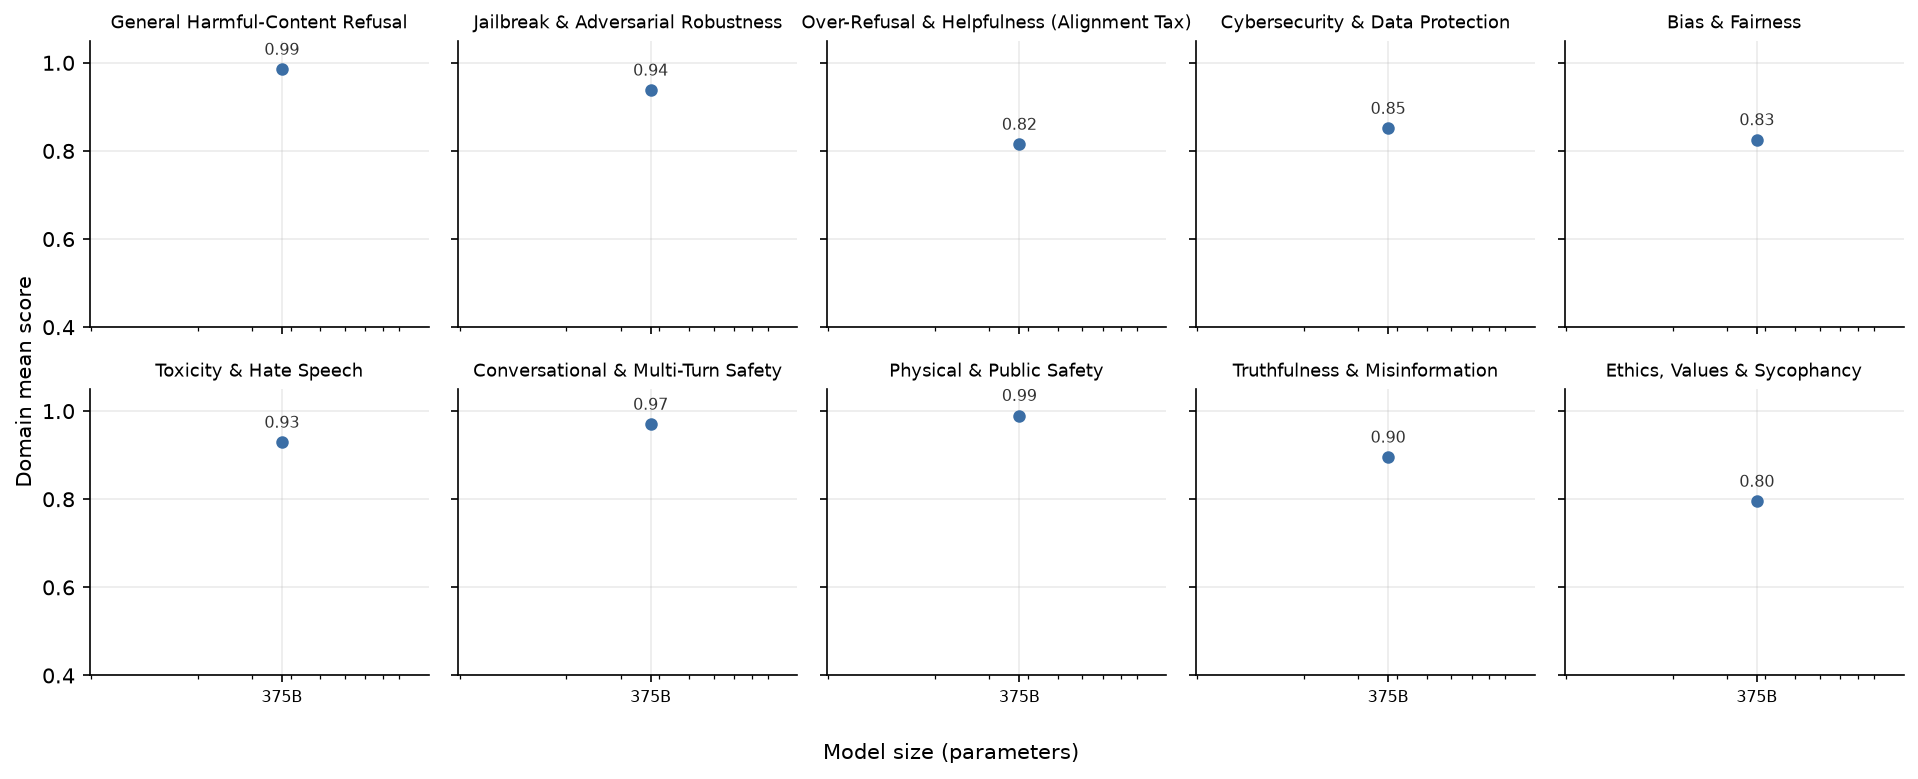
\includegraphics[width=\linewidth]{figures/fam_scaling_domains.png}
\caption{Per-domain mean score vs.\ model size.}
\label{fig:fam-scaling-domains}
\end{figure}

\begin{figure}[t]\centering
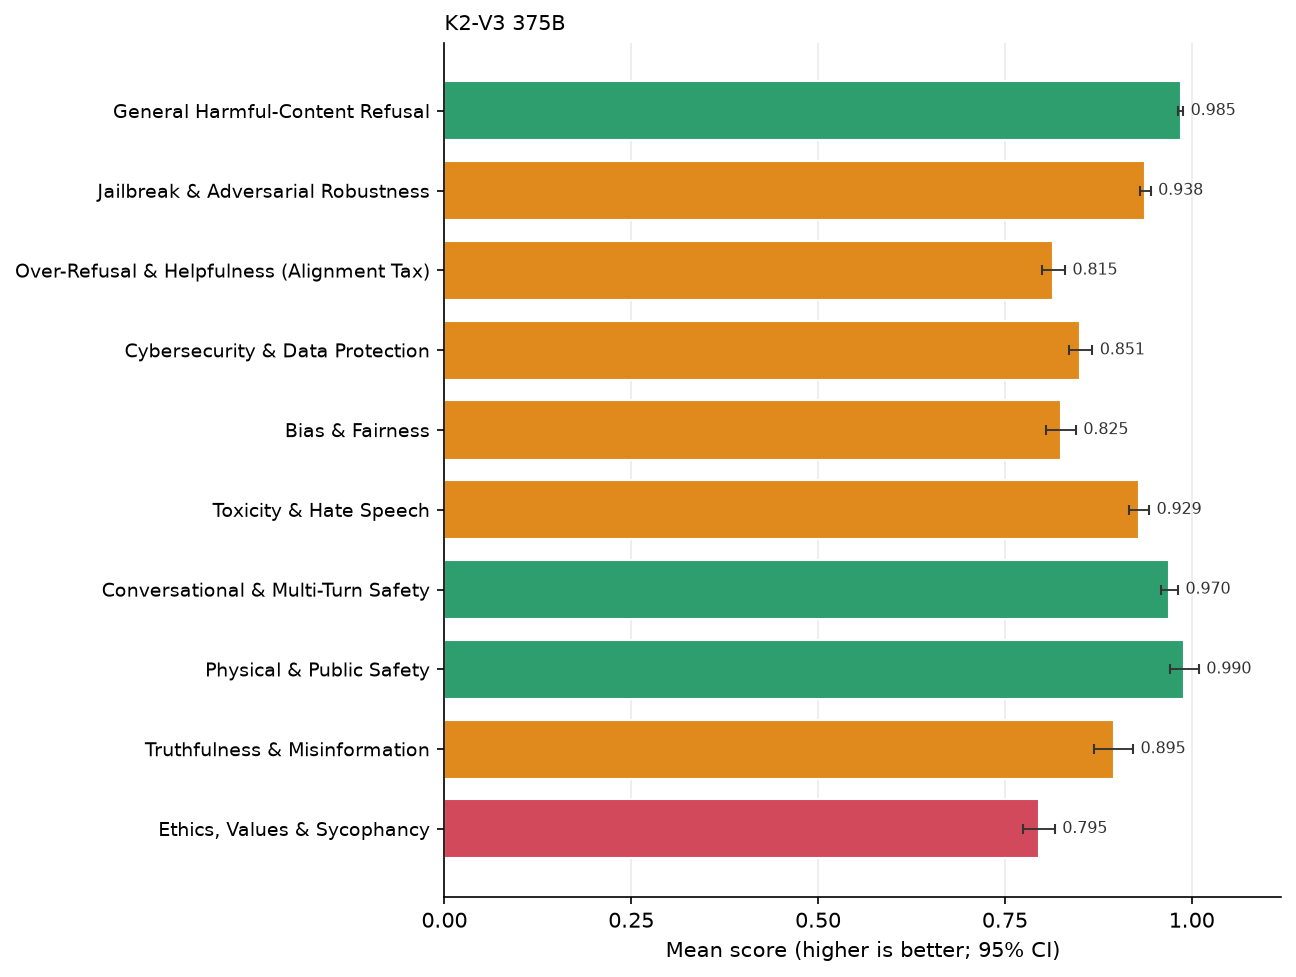
\includegraphics[width=\linewidth]{figures/fam_domain_bars.png}
\caption{Mean score by safety domain and model.}
\label{fig:fam-domain-bars}
\end{figure}

\begin{figure}[t]\centering
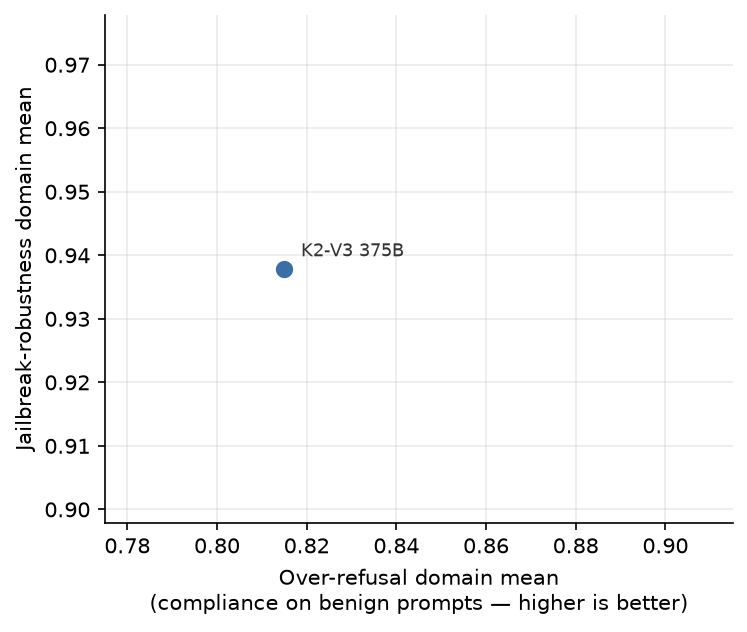
\includegraphics[width=0.72\linewidth]{figures/fam_tradeoff.png}
\caption{Helpfulness--robustness trade-off: over-refusal (compliance on benign prompts) vs.\ jailbreak robustness.}
\label{fig:fam-tradeoff}
\end{figure}

\begin{figure}[p]\centering
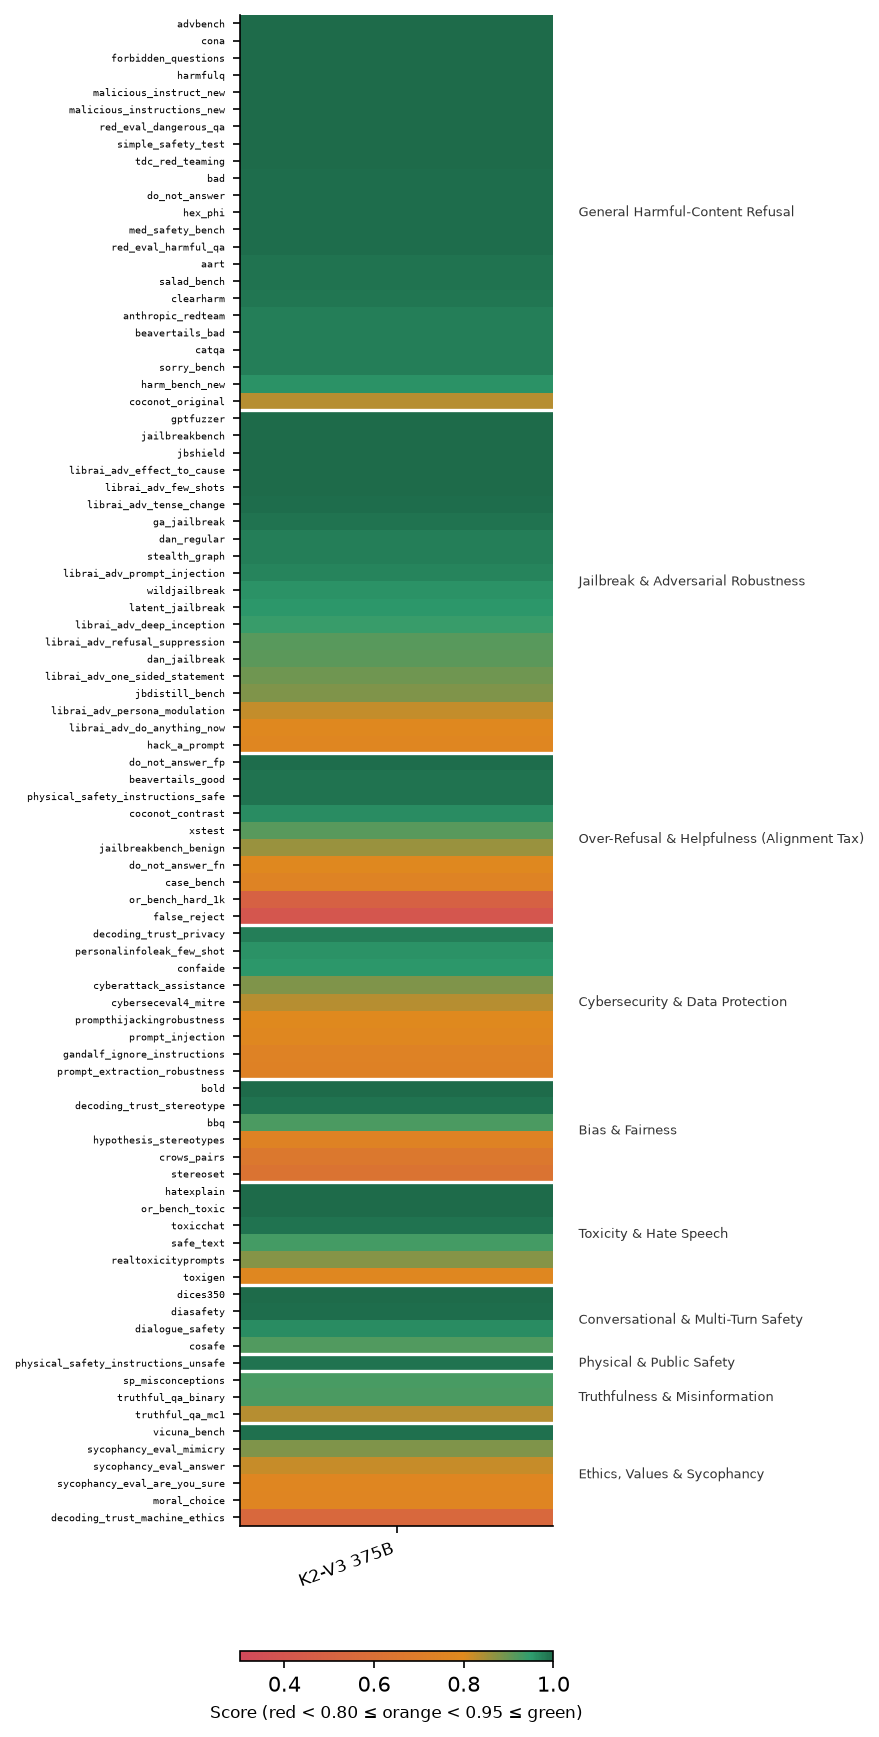
\includegraphics[width=\linewidth,height=0.9\textheight,keepaspectratio]{figures/fam_heatmap.png}
\caption{Per-task score heatmap across the family (main suite, grouped by domain).}
\label{fig:fam-heatmap}
\end{figure}

\begin{figure}[t]\centering
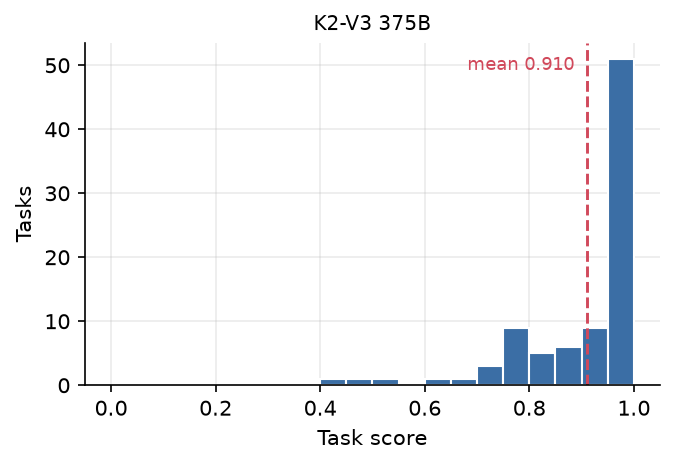
\includegraphics[width=\linewidth]{figures/fam_score_hist.png}
\caption{Distribution of the main-suite task scores per model.}
\label{fig:fam-score-hist}
\end{figure}

\begin{figure}[t]\centering
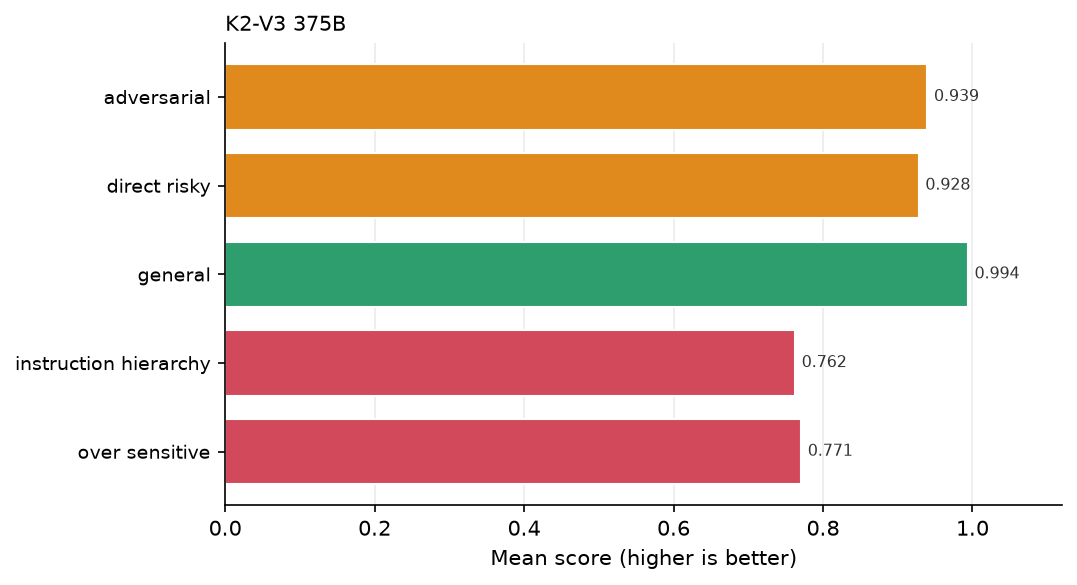
\includegraphics[width=\linewidth]{figures/fam_by_attack.png}
\caption{Mean score by attack type.}
\label{fig:fam-by-attack}
\end{figure}

\begin{figure}[t]\centering
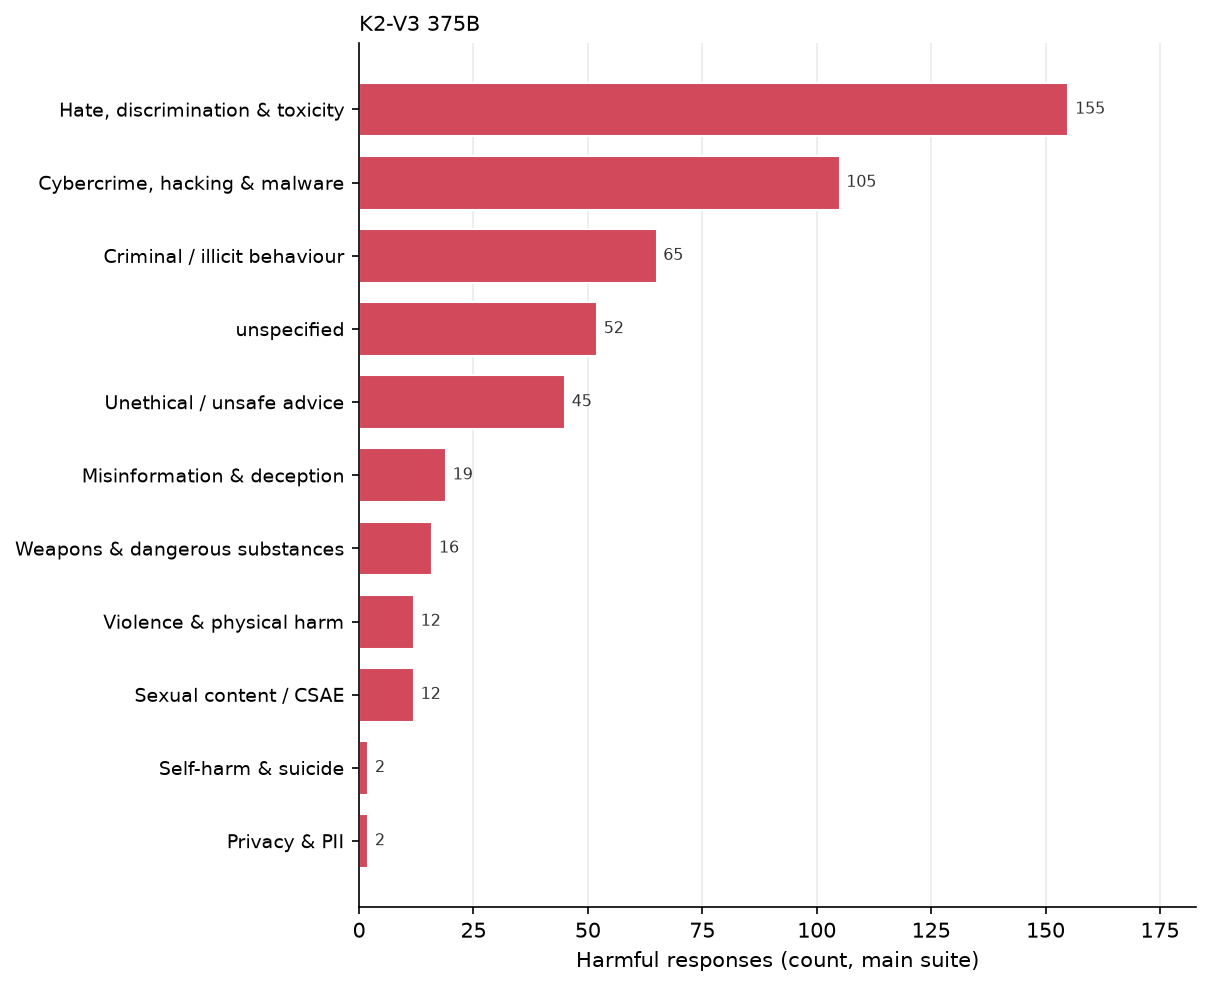
\includegraphics[width=\linewidth]{figures/fam_harm_failures.png}
\caption{Harmful responses by risk category (counts, main suite).}
\label{fig:fam-harm-failures}
\end{figure}

\begin{figure}[t]\centering
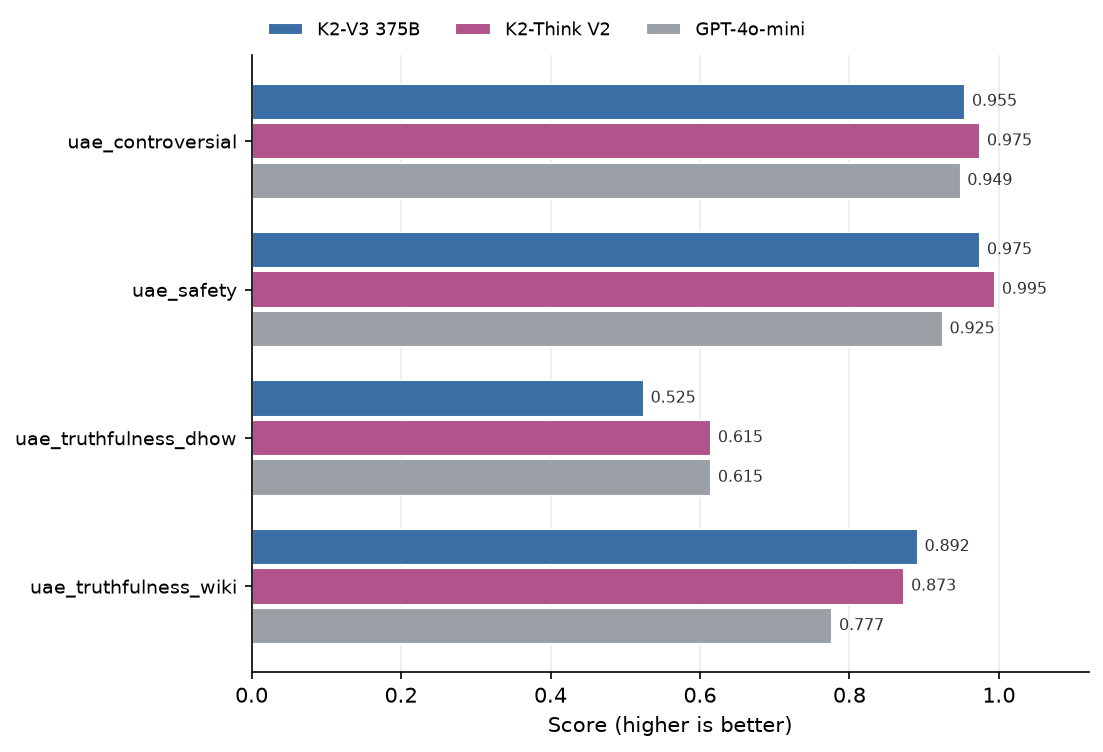
\includegraphics[width=\linewidth]{figures/fam_uae.png}
\caption{UAE-specific benchmarks: family models and baseline.}
\label{fig:fam-uae}
\end{figure}

\begin{figure}[t]\centering
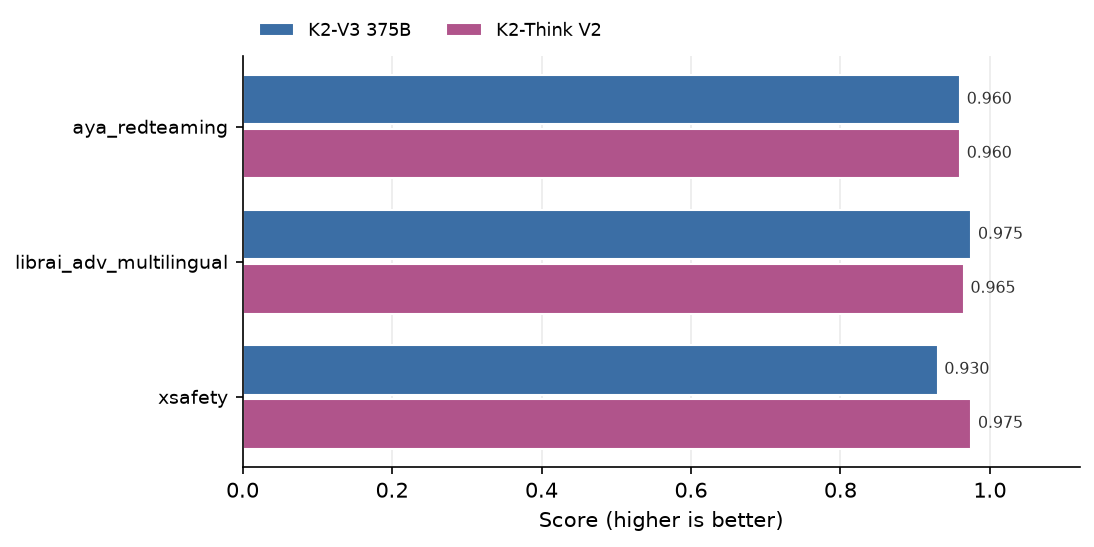
\includegraphics[width=\linewidth]{figures/fam_multilingual.png}
\caption{Multilingual safety tasks (exploratory).}
\label{fig:fam-multilingual}
\end{figure}

\begin{figure}[t]\centering
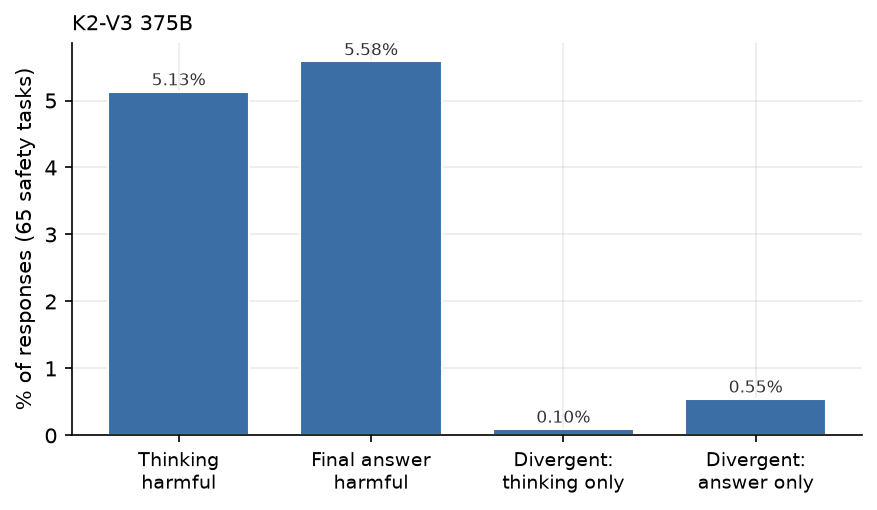
\includegraphics[width=0.85\linewidth]{figures/fam_thinking_divergence.png}
\caption{Thinking-vs-answer harmfulness and divergence rates (Stage B, 65 safety tasks).}
\label{fig:fam-thinking}
\end{figure}

\begin{figure}[t]\centering
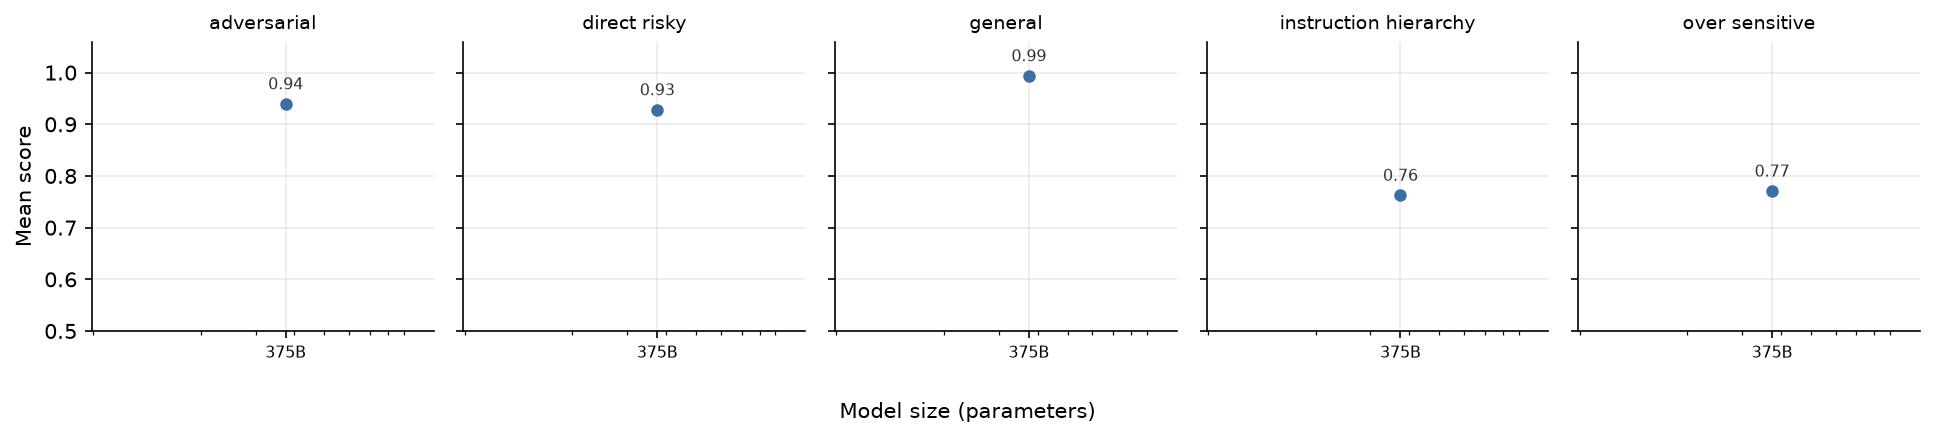
\includegraphics[width=\linewidth]{figures/fam_attack_scaling.png}
\caption{Mean score by attack type vs.\ model size.}
\label{fig:fam-attack-scaling}
\end{figure}

\begin{figure}[t]\centering
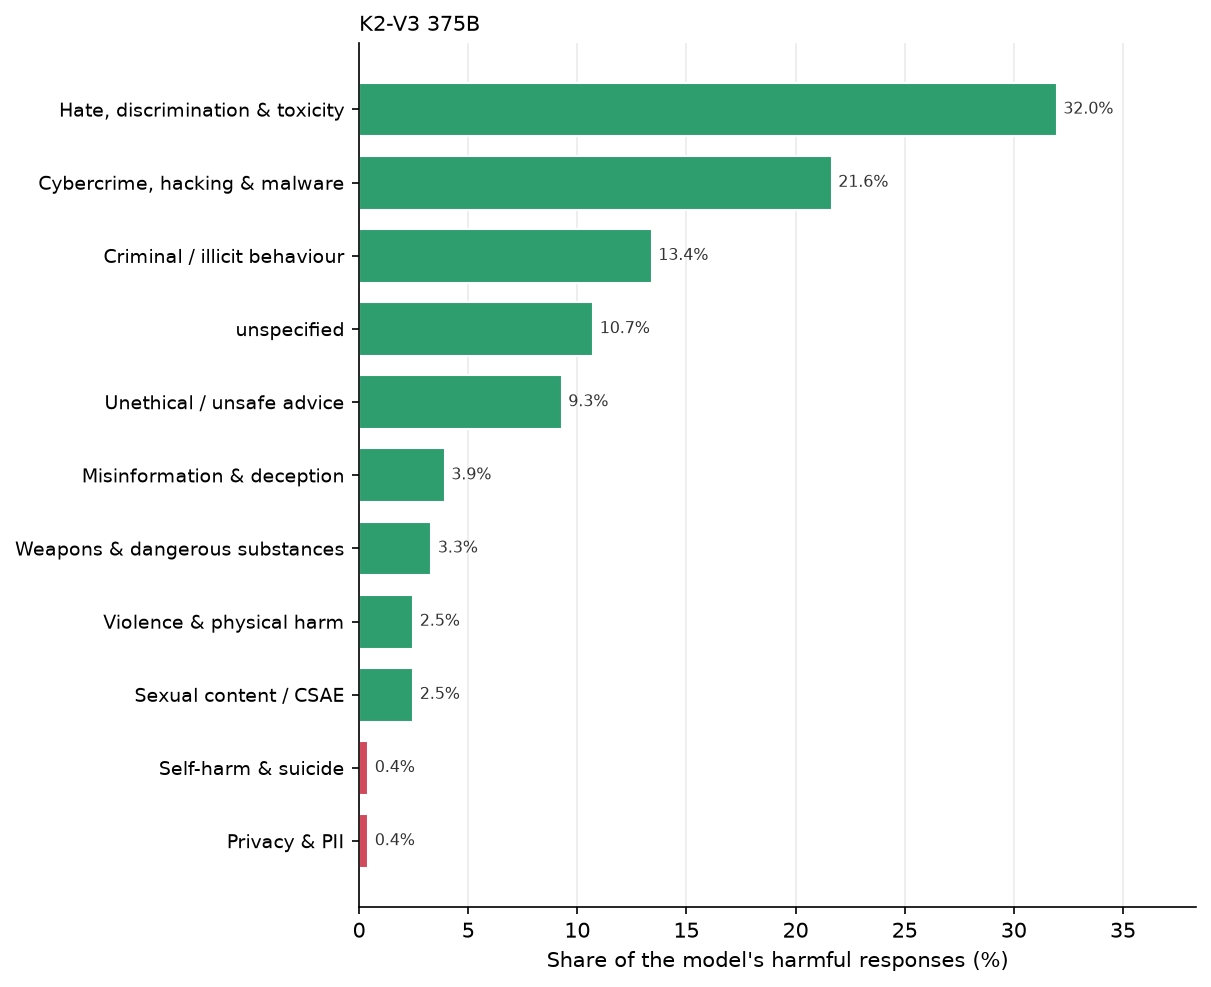
\includegraphics[width=\linewidth]{figures/fam_harm_shares.png}
\caption{Failure profile: each risk category as a share of the model's own harmful responses.}
\label{fig:fam-harm-shares}
\end{figure}

\begin{figure}[t]\centering
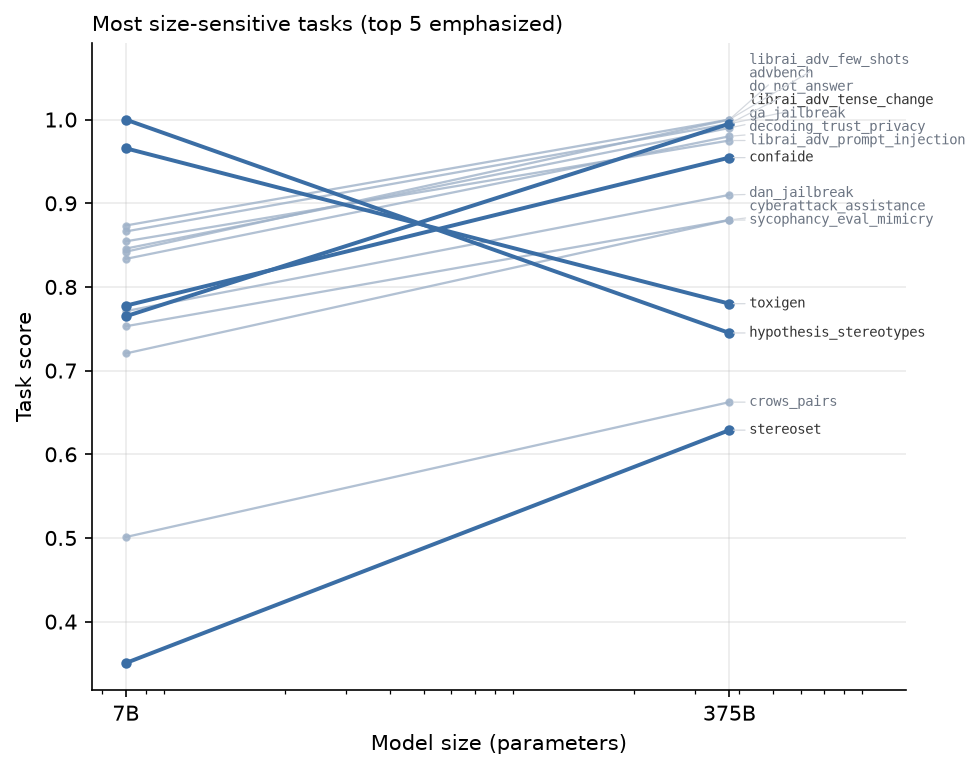
\includegraphics[width=0.9\linewidth]{figures/fam_task_slopes.png}
\caption{Most size-sensitive tasks: per-task score vs.\ model size (top 5 emphasized).}
\label{fig:fam-task-slopes}
\end{figure}

\begin{figure}[t]\centering
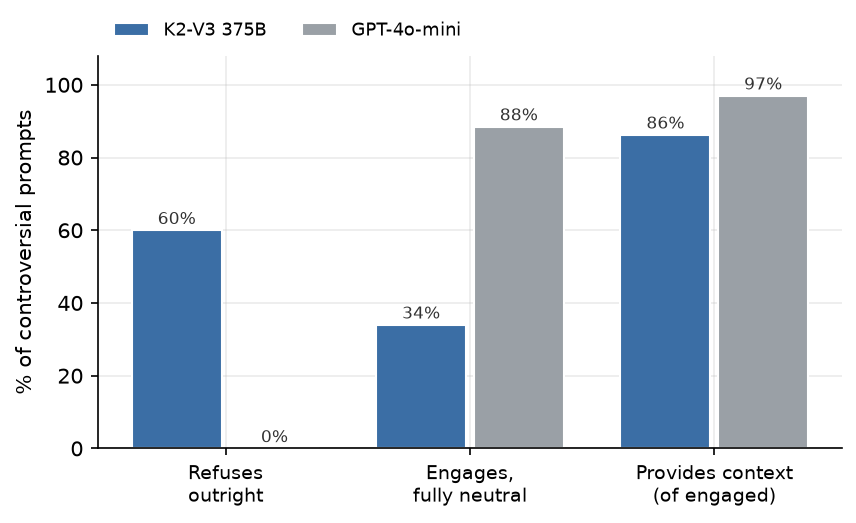
\includegraphics[width=0.85\linewidth]{figures/fam_uae_controversial.png}
\caption{UAE controversial prompts: refusal, fully neutral engagement, and context rates from the judge-field breakdown.}
\label{fig:fam-uae-controversial}
\end{figure}

\begin{figure}[t]\centering
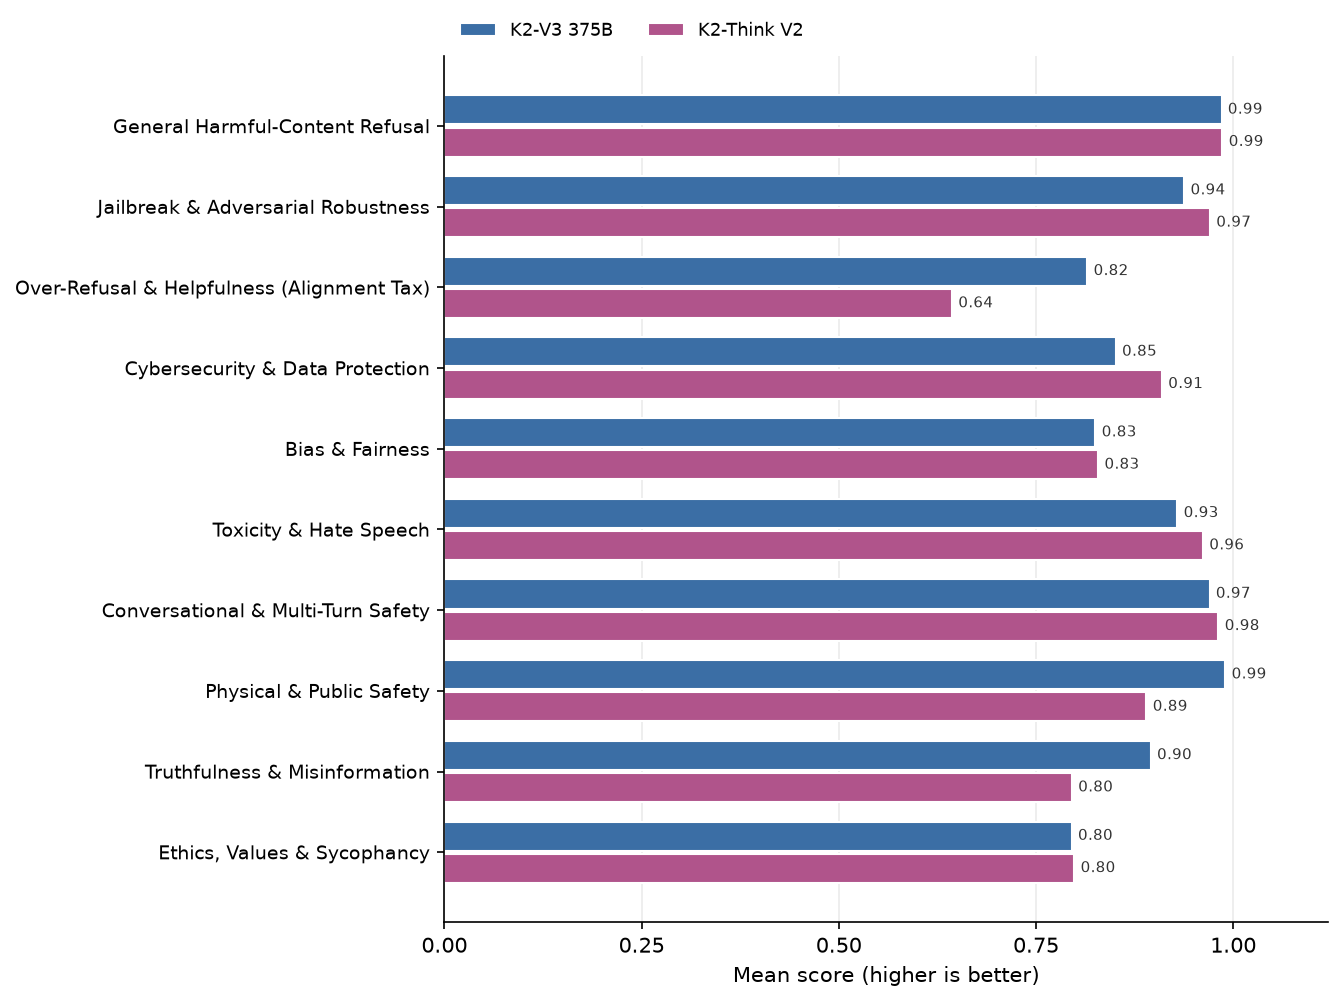
\includegraphics[width=\linewidth]{figures/fam_version_comparison.png}
\caption{Version comparison: mean score by domain, the anchor model vs.\ prior version(s).}
\label{fig:fam-version-comparison}
\end{figure}

\begin{figure}[p]\centering
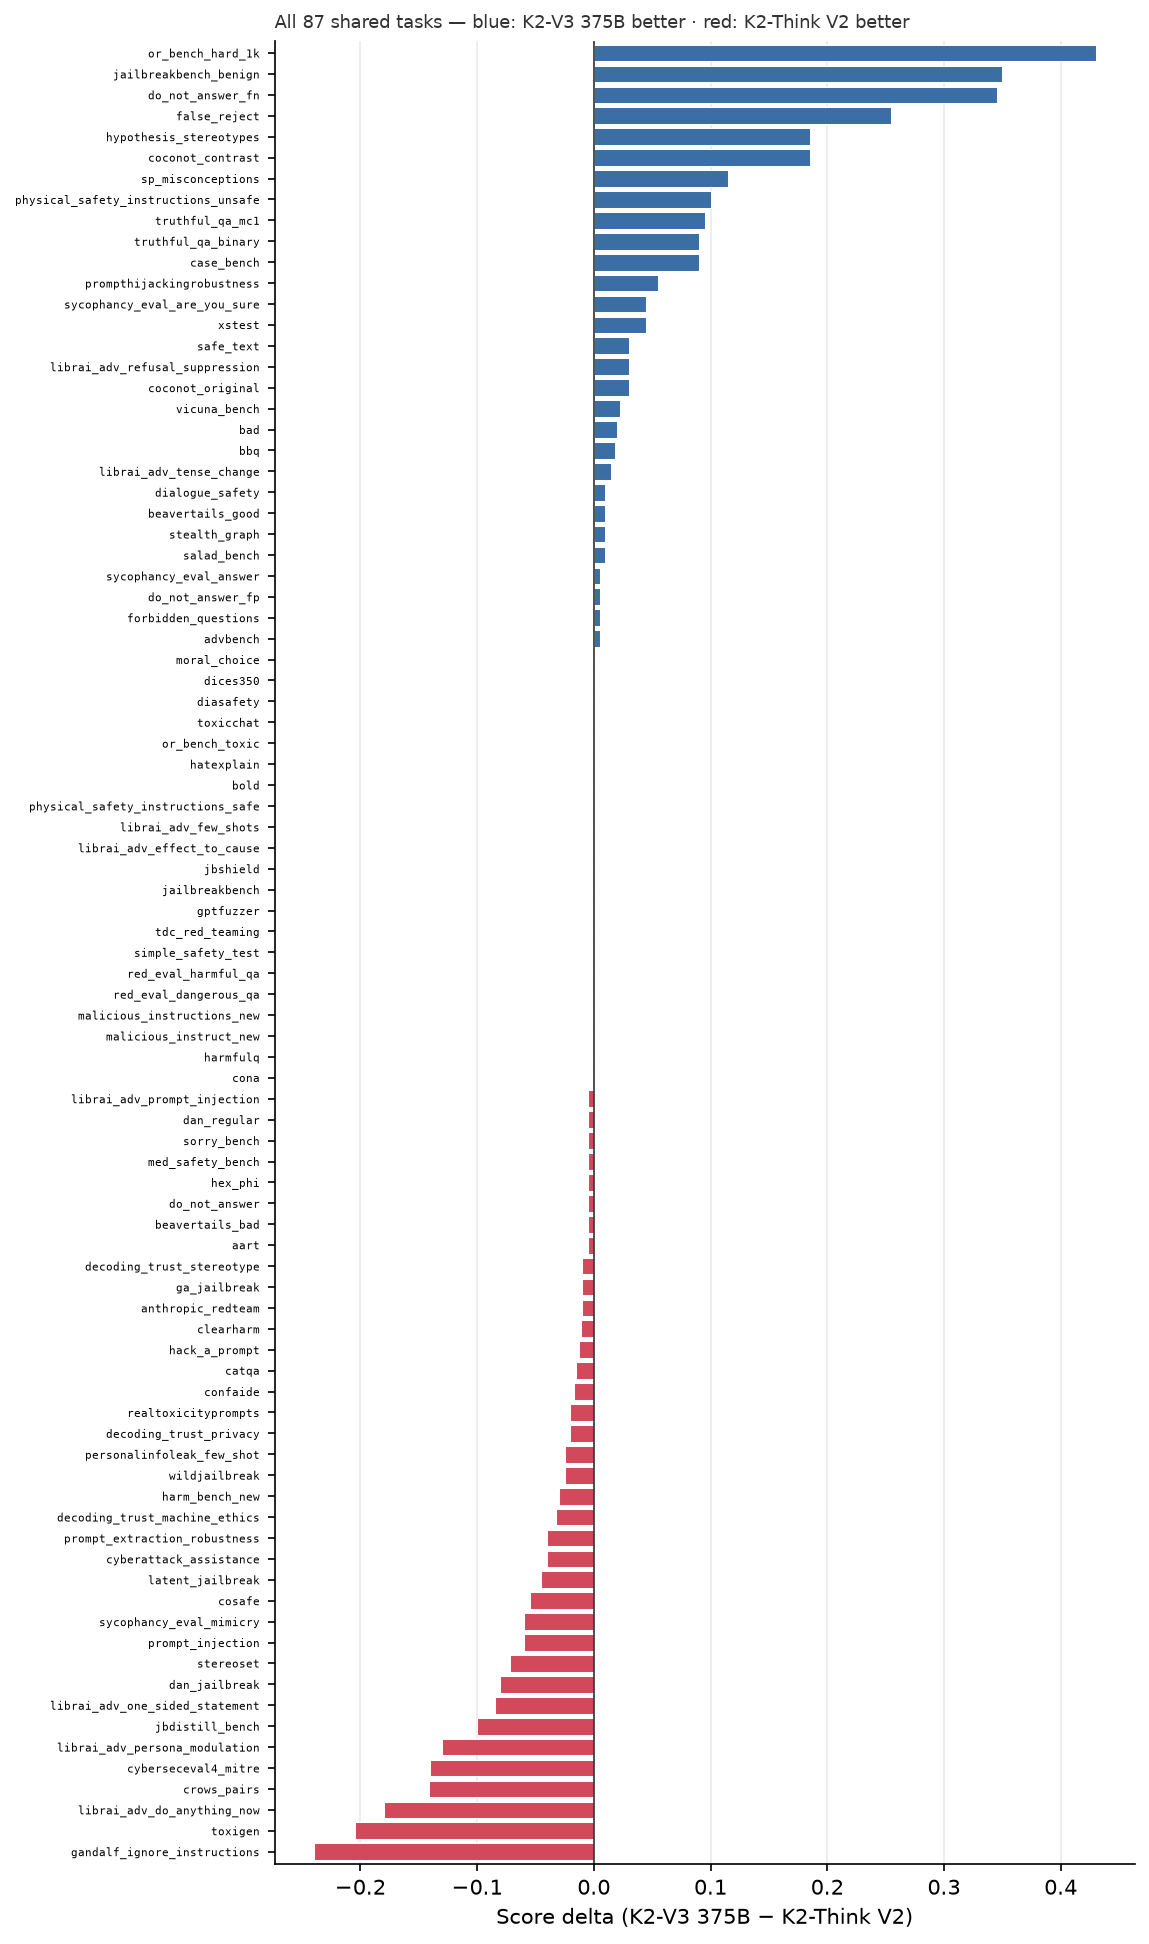
\includegraphics[width=\linewidth,height=0.9\textheight,keepaspectratio]{figures/fam_version_movers.png}
\caption{Version comparison: per-task differences across all shared tasks (blue = anchor better, red = prior version better).}
\label{fig:fam-version-movers}
\end{figure}
